\section{Breaking Symmetries in 8-connected Grids}


Consider a path which enters an empty room $R$ at some perimeter node $m$ and exits at some other
node $n$ located on the opposite side of the room.
On a 4-connected map we can optimally traverse the room by expanding $m$, following
its macro edge to a node $m'$ on the opposite side of $R$ and finally navigating from $m'$ to $n$.
The length of this path is equal to the Manhattan distance between $m$ and $n$ and thus optimal.
However, if the map consists of 8-connected tiles this strategy is no longer optimal.
In particular, the original (unmodified) map may contain a more direct path to $n$ using one or more diagonal
transtions.
\par
We address this problem as follows:
First, we give an offline procedure which adds to $R$ a set of additional macro edges
to facilitate optimal travel between arbitrary pairs of tiles on the perimeter.
Second, we give an online re-insertion procedure which deals with cases where the start or
goal is a tile that has been previously removed.
Finally, we give a proof which shows this method is optimal.
\\ \newline
\textbf{Offline Procedure: }
Our method is a simple 2 step process (shown in Figure \ref{fig-macroedges}):

\begin{enumerate}
\item{First, add a series of macro edges between pairs of perimeter tiles on orthogonal sides of $R$. 
We connect two tiles only if the proposed macro edge represents a path through the interior of $R$ that involves
only diagonal steps. }
\item{Next, add a series of macro edges between pairs of perimeter tiles on opposite sides of $R$.
We connect two tiles only if the proposed macro edge represents a path through the interior of $R$ which is shorter
than any alternative path involving only tiles from the perimeter and possibly one (other) macro edge.
}
\end{enumerate}

\begin{figure}[tb]
       \begin{center}
                       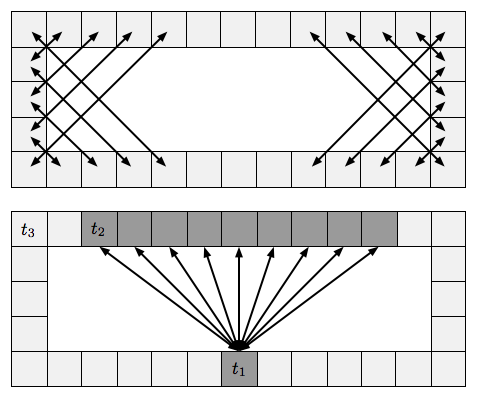
\includegraphics[scale=0.5, trim = 10mm 10mm 10mm 0mm]{diagrams/macroedges.png}
       \end{center}
	\vspace{-3pt}
       \caption{(Top) Macro edges between tiles on orthogonal sides of an empty room. 
(Bottom) Each tile on the perimeter is connected to a set of tiles on the opposite side of the room.
Dominated edges are skipped; in this case the path $\lbrace t1, t2, t3 \rbrace$
dominates the proposed edge $(t1, t3)$.}
       \label{fig-macroedges}
\end{figure}
We claim this method preserves optimality when traversing arbitrary rooms in an 8-connected grid map.
\begin{lemma}
\label{lemma-rooms}
Let $R$ be an empty rectangular room in an 8-connected grid map.
Further, let $m$ and $n$ be two locations along its perimeter.
Then, $m$ and $n$ can be connected optimally through a path that mentions only nodes on the perimeter of $R$ and
possibly involves one macro edge.
\end{lemma}

\begin{proof}
There are three cases to consider:
\begin{enumerate}
\item{$m$ and $n$ are on the same side of the perimeter.}
\item{$m$ and $n$ are on orthogonal sides of the perimeter.}
\item{\label{lemma-rooms-step3} $m$ and $n$ are on opposite sides of the perimeter.}
\end{enumerate}
In the first case we can simply walk along the perimeter from $m$ to $n$; the optimality of this path is immediate. 
In the second and third case we argue as follows: if $m$ and $n$ are not connected by a macro edge
we can walk along the perimeter from $m$ to an intermediate node $m'$ and follow a macro edge to a node $n'$ on the 
same side of the perimeter as $n$. Finally, we walk along the perimeter from $n'$ to $n$.
The length of this path is equal to the octile distance between $m$ and $n$ and therefore optimal
\footnote{Note that in some cases $m' = m$ or $n' = n$ (or both).}.
\end{proof}

\noindent
\textbf{Online Insertion:}
It is often the case that a tile from the interior of an empty room is required as a start or goal location for an
agent. 
To handle such situations we give an online procedure that temporarily re-inserts tiles back into the map for the duration
of a search. 
Our method is a variation on the re-insertion alogorithm described in \cite{harabor10}. It proceeds as follows:

\begin{enumerate}
\item{If the start and goal are interior nodes in the same room no insertion is necessary; an optimal
path is trivially available. }
\item{If the start and goal are not in the same room, add to $R$ a series of non-dominated macro edges that connects
the inserted tile to a set of nodes on each side of the room's perimeter. This is similar to Step 2 of our offline procedure.}
\end{enumerate}
%It is possible to identify, in constant time, the set of tiles which the start or goal must be connected to.
%Further, in an efficient implementation, we could generate these neighbours on the fly.
%This means the time complexity associated with insertion can be as low as $O(1)$.
\begin{lemma}
\label{lemma-insertion}
Let $R$ be an empty rectangular room in an 8-connected grid map.
For any nodes $m$, $n$, with $m$ a re-inserted interior node and $n$ a node on the perimeter, it is always possible to
find an optimal length path which mentions no interior nodes except for $m$.
\end{lemma}
The (omitted) proof uses a similar argument to the one given for Step \ref{lemma-rooms-step3} of Lemma \ref{lemma-rooms}.

%We claim that using the temporary macro edges added by this algorithm it is possible to travel optimally from the start or goal 
%location to any tile on the perimeter of the start or goal room. 
\par \noindent
\newline
\textbf{Optimality:} We claim the symmetry elimination procedure outlined in this section is sufficient to guarantee
that A*, running on a modified 8-connected grid map, will always find an optimal length solution if one exists.
Our (omitted) proof follows from Lemma \ref{lemma-rooms} and Lemma \ref{lemma-insertion}.
It is based on the observation that for every segment of an optimal length path, which enters a room at some tile $m$
and exits at some tile $n$, there is an equivalent length path that mentions only nodes from the perimeter of that room 
and possibly one macro edge.
